\tikzstyle{block} = [draw, fill=blue!20, rectangle, 
    minimum height=3em, minimum width=3em]
\tikzstyle{sum} = [draw, fill=blue!20, circle, node distance=1cm]
\tikzstyle{sum2} = [draw, fill=blue!20, circle, node distance=1cm]
\tikzstyle{input} = [coordinate]
\tikzstyle{output} = [coordinate]
\tikzstyle{out} = [coordinate]
\tikzstyle{out2} = [coordinate]
\tikzstyle{pinstyle} = [pin edge={to-,thin,black}]

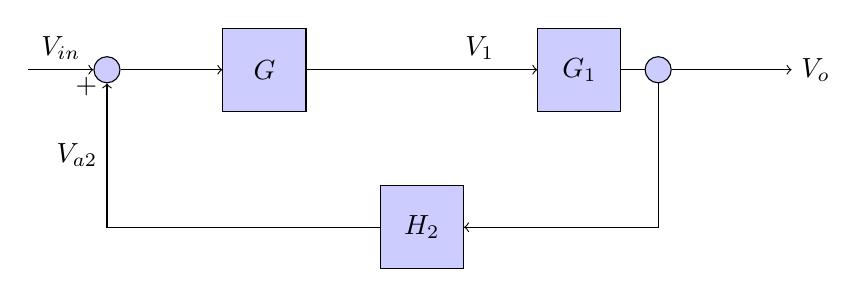
\begin{tikzpicture}[auto, node distance=2cm]
    \node [input, name=input] {};
    \node [sum, right of=input] (sum) {};
    \node [block, right of=sum] (controller) {$G$};
    \node [output, right of=controller] (output) {};
    \node [block, right of= output](controller2){$G_1$};
    \node [sum2,right of=controller2](sum2){};
    \node [block, below of=output] (feedback) {$H_2$};
    \node[right of = sum2](out2){$V_o$};
    \draw [draw,->] (input) -- node {$V_{in}$} (sum);
    \draw [->] (sum) -- node {} (controller);
    \draw [-] (controller) -- node {}(output);
    \draw [->] (output) --node{$V_1$} (controller2);
    \draw [-] (controller2) -- node{} (sum2);
   \draw[->] (sum2) |- (feedback);
    \draw[->] (sum2) -- (out2);
    \draw [->] (feedback) -| node[pos=0.99]{$+$}  node [near end] {$V_{a2}$} (sum);
\end{tikzpicture}
